%                                                                 aa.dem
% AA vers. 8.2, LaTeX class for Astronomy & Astrophysics
% demonstration file
%                                                       (c) EDP Sciences
%-----------------------------------------------------------------------
%
%\documentclass[referee]{aa} % for a referee version
%\documentclass[onecolumn]{aa} % for a paper on 1 column  
%\documentclass[longauth]{aa} % for the long lists of affiliations 
%\documentclass[rnote]{aa} % for the research notes
%\documentclass[letter]{aa} % for the letters 
%\documentclass[bibyear]{aa} % if the references are not structured 
% according to the author-year natbib style

%
\documentclass{aa}  

%
\usepackage{graphicx}
%%%%%%%%%%%%%%%%%%%%%%%%%%%%%%%%%%%%%%%%
\usepackage{txfonts}
%%%%%%%%%%%%%%%%%%%%%%%%%%%%%%%%%%%%%%%%
\usepackage{hyperref}
\pdfoutput=1
\usepackage{amsfonts}
\usepackage{amsmath}
\usepackage{amssymb}
\usepackage{xcolor}
\usepackage{enumitem}
\usepackage{graphicx}
\usepackage{gensymb}
\usepackage{fancyhdr}
\usepackage{times}
\usepackage{ulem}
%\usepackage{caption}
\usepackage{subcaption} 
\usepackage{float} 



\begin{document} 


   \title{A K1000 Shear Statistics Paper}

   \subtitle{or ``How I learned to stop worrying and love systematics"}

   \author{Author-1
          \inst{1}
          \and
          the KiDS Collaboration\inst{2}\thanks{bengib@roe.ac.uk}
          }

   \institute{Scottish Universities Physics Alliance, Institute for Astronomy, University of Edinburgh, Blackford Hill, Edinburgh, EH9 3HJ, UK \\ \and
   University of Life\\
    }

 %  \date{Received September 15, 1996; accepted March 16, 1997}

% 5 {} token are mandatory
 
  \abstract
  % context heading (optional)
  % {} leave it empty if necessary  
   {Lensing measurements are a powerful cosmological probe but are subject to various data-related systematics.}
  % aims heading (mandatory)
   {To demonstrate the reliability of the shear measurements with the KiDS DR4.}
  % methods heading (mandatory)
   {List of tests how we do this.}
  % results heading (mandatory)
   {We find everything is hunky dory.}
  % conclusions heading (optional), leave it empty if necessary 
   {}

   \keywords{observations: galaxies: general -– astronomical data bases: surveys -– cosmology: large-scale structure of Universe}

   \maketitle
%
%________________________________________________________________

\section{Introduction}

The coherent statistical correlations in the shapes of background  galaxies, a consequence of weak gravitational lensing of the galactic light by foreground large-scale structure, are encoded with cosmological information. Measurement of these correlations, a method known as \textit{cosmic shear}, thus stands as a powerful means to infer cosmological parameters. Indeed, recent analyses from `Stage III' weak lensing teams, the Kilo-Degree Survey \citep[KiDS]{Hildebrandt_etal_2018}, the Dark Energy Survey \citep[DES]{DES_Cosmic_Shear_Yr1} and the Hyper-Suprime Cam Collaboration \citep[HSC]{Hamana_etal_2019}, using several hundreds to thousands of square-degrees of sky coverage, have yielded unprecedented precision in the cosmic shear constraints on the clustering parameter $S_8 = \sigma_8 \sqrt{ \Omega_{\rm m}/0.3 }$, where $\sigma_8$ is the amplitude of matter fluctuations and $\Omega_{\rm m}$ is the matter energy density. The success of these investigations builds upon the work of previous generations of cosmic shear analyses, from the tens of square-degrees observed by Stage I surveys including SDSS \citep{Hirata_etal_2004}, VIRMOS-Descart \citep{vanWaerbeke_etal_2005}, CTIO \citep{Jarvis_etal_2006} and COSMOS \citep{Schrabback_etal_2007}, to the Stage II surveys of up to some hundreds of square-degrees, for example, CFHTLenS \citep{Heymans_etal_2013}, further observations by SDSS \citep{Lin_etal_2012,Huff_etal_2014}, RCSLenS \citep{Hildebrandt_etal_2016b} and DLS \citep{Jee_etal_2016}.  

    

\begin{itemize}

\item But cosmic shear is hard - weak signal, PSF, shape measurement etc.

\item Summarise shear estimation biases: noise, model and selection bias. Multiplicative and additive shear biases.

\item KiDS analysis pipeline. 

\end{itemize}

\section{Data}

The Kilo-Degree Survey is an ESO public survey comprising 1350 deg$^2$ of deep imaging in the $ugri$ bands from the 2.3 m VLT Survey Telescope \cite[VST]{Capaccioli_Schipani_2011, Capaccioli_etal_2012}. The images are captured by the wide-field optical camera, OmegaCAM \citep{Kuijken_2011}, featuring 268 million pixels across 32 CCD detectors, with a 1.013$\times$1.020 deg$^2$ field of view. This paper focuses on the first 1000 deg$^2$ of $r$-band observations \citep[K1000]{Kuijken_etal_2019}, used for shear estimation and taken during the survey's dark time with the best seeing conditions ($\rm{FWHM} < 0.8 \, \rm{arcsec}$). The remaining $ugi$ bands, combined with five near-infrared bands, $ZYJHK_{\rm s}$, from the VISTA Kilo-degree INfrared Galaxy survey \citep[VIKING]{Edge_etal_2013}, supplement the $r$-band in providing galaxy colours for photometric redshift estimation, as discussed in \cite{Hildebrandt_etal_2018} and \cite{Kuijken_etal_2019}. Multiple dithered exposures are taken in each band to minimise the effect of CCD gaps and incident cosmic rays. The raw images taken at the telescope feature a number of imperfections which require dedicated processing to achieve science-ready data products. We perform this processing on the $r$-band imaging using the THELI pipeline \citep{Erben_etal_2005, Schirmer_etal_2013}, whereas the processing of the bands used in photometric redshift estimation is conducted via the ASTROWISE system \citep{Begeman_etal_2013}; we refer the reader to \cite{Hildebrandt_etal_2016} and \cite{Kuijken_etal_2019} for further details.  
	




\section{\textit{lens}fit-{\sc{Metacalibration}} }

    \subsection{Optimal weighting}

\section{PSF estimation} \label{sec:PSF_Estimation}

	The atmospheric PSF, the PSF due to the imperfect response of the CCD pixels to incident photons, and that of the sub-optimal CCD charge diffusion, can all be considered as contributors to the overall effective PSF one must correct for. The PSF is modelled based on the light profile of calibration stars at various positions in the field of view. The model is then interpolated to other locations on the sky, such that galaxy shapes can be correct for this effect \citep[see, for example,][]{Berge_etal_2012, Gentile_etal_2013, Kitching_etal_2013, Lu_etal_2017}.
	
	\subsection{Selection of PSF stars}
	
	\subsection{PSF modelling}
	
	
	
	For the KiDS imaging, a PSF model, taking the form of 2-dimensional polynomial of order $n$, is fit across the whole field of view, with the coefficients up to order $n_{\rm c}$ given freedom to vary between each of the 32 CCD detectors in OmegaCAM.  This allows for flexible spatial variation (including discontinuities) in the PSF. The total number of model coefficients per field of view is given by \citep{Kuijken_etal_2015},
	\begin{equation}
	N_{\rm coeff} = \frac{1}{2} \left[ (n+1)(n+2) + (N_{\rm D}-1)(n_{\rm c} +1)(n_{\rm c}+2) \right] \,,
	\label{eqn:PSFModel_KiDS}
	\end{equation}
	where $N_{\rm D}=32$ is the number of CCD detectors in OmegaCAM. Additionally, the flux and position of each calibration star are also allowed to vary in the PSF fitting, permitting further flexibility to the model. The total number of coefficients is large, but is sufficiently well constrained by the the number of data points, equal to the number of pixels times the number of identified stars per exposure. The model is initially fit to stars identified in data from the \cite{Gaia_etal_2018} down to the magnitude limit of this survey, and then refined using fainter stars in the KiDS imaging via the method in \cite{Kuijken_etal_2019}.   
	
	
	Errors in estimating the size and shape of the PSF result in multiplicative and additive shear biases. The PSF impacts shear estimation also via its spatial correlations. Whereas the effect these have on the $\xi_-$ correlation function is negligible, the contribution to $\xi_+$ can be quantified using the $\rho$ statistics \citep{Rowe_2010, Jarvis_etal_2016}, 
	\begin{equation}
	\begin{split}
	\rho_1(\theta) & \equiv \langle \delta e_{\rm PSF}^*(\boldsymbol{x}) \, \delta e_{\rm PSF}(\boldsymbol{x}+\boldsymbol{\theta}) \rangle \,, \\
	\rho_2(\theta) & \equiv \langle e_{\rm PSF}^*(\boldsymbol{x}) \, \delta e_{\rm PSF}(\boldsymbol{x}+\boldsymbol{\theta}) \rangle \,, \\
	\rho_3(\theta) & \equiv \Bigg\langle \left( e_{\rm PSF}^* \frac{\delta T_{\rm PSF}}{T_{\rm PSF}} \right)   (\boldsymbol{x}) \, \left( e_{\rm PSF} \frac{\delta T_{\rm PSF}}{T_{\rm PSF}} \right)(\boldsymbol{x}+\boldsymbol{\theta}) \Bigg\rangle \,, \\	
	\rho_4(\theta) & \equiv \Bigg\langle \delta e_{\rm PSF}^* (\boldsymbol{x}) \, \left( e_{\rm PSF} \frac{\delta T_{\rm PSF}}{T_{\rm PSF}} \right)(\boldsymbol{x}+\boldsymbol{\theta}) \Bigg\rangle \,, \\	
	\rho_5(\theta) & \equiv \Bigg\langle \delta e_{\rm PSF}^* (\boldsymbol{x}) \, \left( e_{\rm PSF} \frac{\delta T_{\rm PSF}}{T_{\rm PSF}} \right)(\boldsymbol{x}+\boldsymbol{\theta}) \Bigg\rangle \,, \\	
	\end{split}
	\label{eqn:RhoStats}
	\end{equation}
	where $e_{\rm PSF}$ and $\delta e_{\rm PSF} \equiv e_{\rm PSF} - e_{\rm model}$ are the ellipticity of the PSF and its residual, measured at the positions of stars, respectively. $T_{\rm PSF}$ is the size of the PSF, taken to be the trace of the second moments of the surface brightness profile, $I(\boldsymbol{\theta})$, given by \citep{Bartelmann_Schneider_2001},
\begin{equation}
Q_{ij} = \frac{\int d^2\boldsymbol{\theta} \, w[I(\boldsymbol{\theta})] \, I(\boldsymbol{\theta}) \, \theta_i\theta_j }{ \int d^2\boldsymbol{\theta} \, w[I(\boldsymbol{\theta})] \, I(\boldsymbol{\theta}) } \,,
\label{eqn:Moment_Brightness_Profile}
\end{equation} 
where $w[I(\boldsymbol{\theta})]$ is a weight function, for example, a Heaviside step function centred on a limiting isophote, and $\delta T_{\rm PSF} \equiv T_{\rm PSF} - T_{\rm model}$. The correlations are measured with pairs of stars separated by the angle $\theta$. The additive systematic error to $\xi_+$ caused by finite $\rho$ contributions is given by \citep{Jarvis_etal_2016},
	\begin{equation}
\delta \xi_+(\theta) = { \Bigg\langle \frac{T_{\rm PSF }}{T_{\rm gal}} \Bigg\rangle}^2 \left(\rho_1(\theta) + \rho_3(\theta) + \rho_4(\theta) \right) - \alpha \Bigg\langle \frac{T_{\rm PSF}}{T_{\rm gal}} \Bigg\rangle \left( \rho_2(\theta) + \rho_5(\theta) \right) \,,
	\label{eqn:RhoStats_Bias}
\end{equation}
	where $T_{\rm gal}$ is the intrinsic galaxy size, unconvolved with the PSF. $\alpha$ is the amount of PSF ``leakage", with contributions, $a$ and $b$, which give rise to an additive shear bias,
	\begin{equation}
	c_i = a_i e_{{\rm model},i} + b_i \delta e_{{\rm PSF},i} \,,
	\end{equation}
		where $i$ denotes the component of the ellipticity. The first term is associated with the deconvolution of the PSF from the galaxy ellipticities, such that $a \neq 0$ if this is done imperfectly. The second term is associated with how well the model fits the true effective PSF. A value of order $-1$ is expected for $b$, since PSF model errors will propagate into an error of the same magnitude, but opposite sign, in the shear \citep{Paulin-Henriksson_etal_2008}. These terms can be estimated from the gradient of the galaxy ellipticities, and the PSF residuals, both with respect to those of the PSF model \citep{Zuntz_etal_2018}. 
		
	We compute the $\rho$ statistics for four different PSF models characterised by the polynomial orders $n:n_{\rm c}$ (see equation \ref{eqn:PSFModel_KiDS}): 3:1, 4:1, 3:2 and 5:1. We find that although the PSF is accurately modelled by all polynomial orders, as determined by the low-level $\rho$ correlations, the 3:1 model, used for the previous KiDS data release in \cite{Kuijken_etal_2015}, does not perform as well as the other three, for which the results are very similar. Therefore, we adopt the 4:1 model for K1000, given it has the least number of coefficients of the remaining options.
	

	Figure \ref{fig:RhoStats} shows the $\rho$ statistics and the corresponding systematic bias, $\delta\xi_+$, for the K1000 imaging assuming 4:1 PSF model an a very large amount of PSF leakage, $\alpha=0.03$, arbitrarily selected as being $\sim 30$ times the additive bias in the previous data release, KiDS-450 \citep{Hildebrandt_etal_2016}. The yellow band, included in the plot to guide the eye, shows $\pm$10\% of the weakest of the $\xi_+$ measurements from the KiDS tomographic bins. This corresponds to the photometric redshift range $z_{\rm B} \in [0.1,0.3]$. The error bars (too small to be seen in some cases) come from a jackknife resampling, whereby the field is divided into $N_{\rm jk}$ segments which are removed one-by-one, with the $\rho$ statistics being calculated from the remaining $N_{\rm jk}-1$ segments at each iteration.

\begin{figure}
\begin{center}
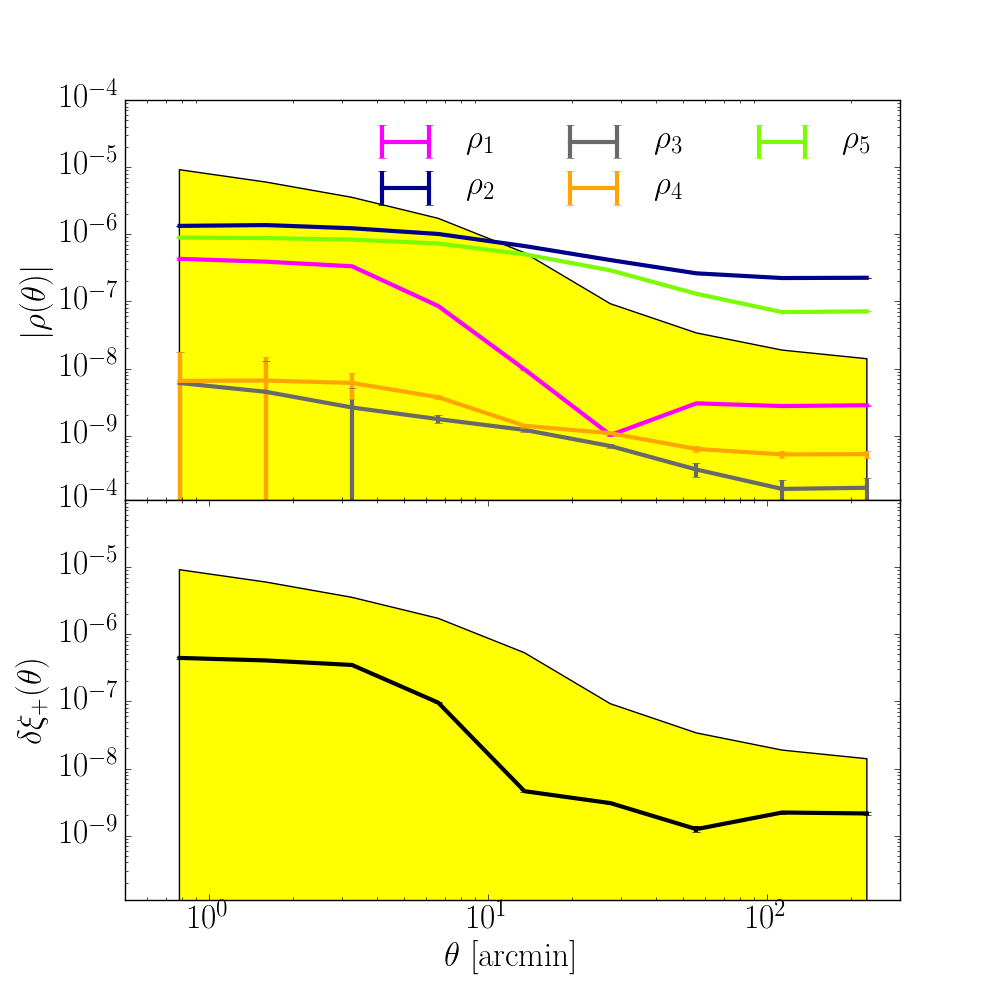
\includegraphics[width=0.5\textwidth]{{Figures/Plot_Overall-rho+_CovPatches7x7}.png} 
\caption{The $\rho$ statistics (upper panel; see equation \ref{eqn:RhoStats}) and corresponding bias on $\xi_+$ (lower panel; equation \ref{eqn:RhoStats_Bias}), assuming a very high level of PSF leakage, $\alpha=0.03$, arbitrarily selected. The yellow band, serving as a general guide rather than a requirement, shows $\pm$10\% of the weakest of the $\xi_+$ signals measured in each of the tomographic bins. This corresponds to the photometric redshift range $z_{\rm B} \in [0.1,0.3]$. The errors (too small to be seen in some cases) come from jackknife resampling.} \label{fig:RhoStats}
\end{center}
\end{figure}



\section{Tests of the shear measurements}

    \subsection{Spatial test}
    e.g. mean ellipticity across the chips, tangential shear around centres of fields
    
    \begin{figure*}
\begin{center}
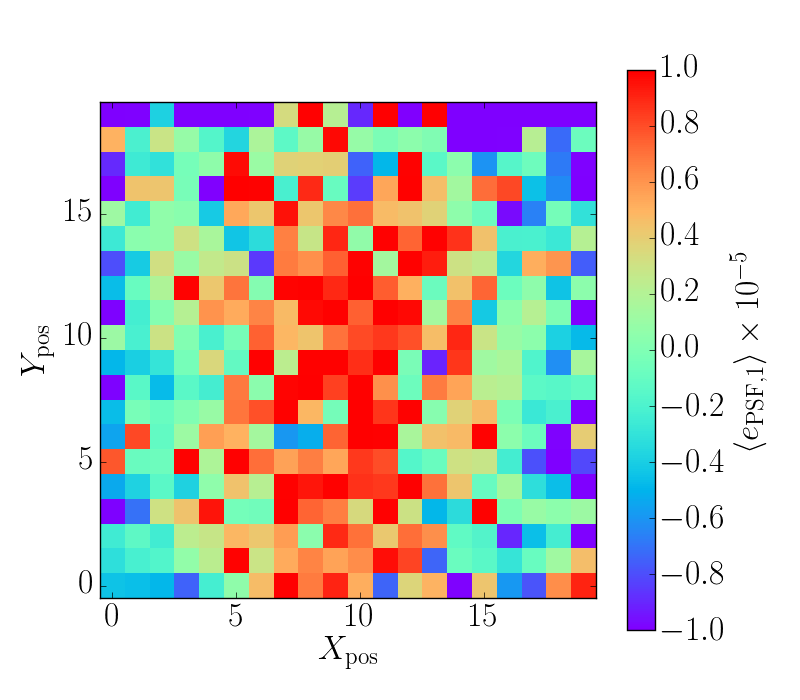
\includegraphics[width=0.49\textwidth]{{Figures/KAll.BlindA.MeanPSFe1_VS_XY.ZBcutNone}.png}
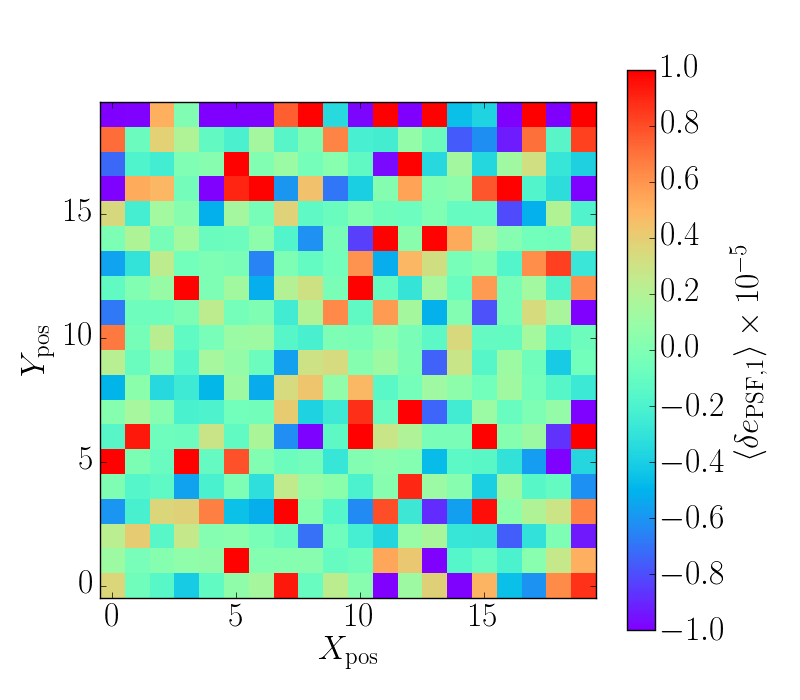
\includegraphics[width=0.49\textwidth]{{Figures/KAll.BlindA.MeandeltaPSFe1_VS_XY.ZBcutNone}.png} \\
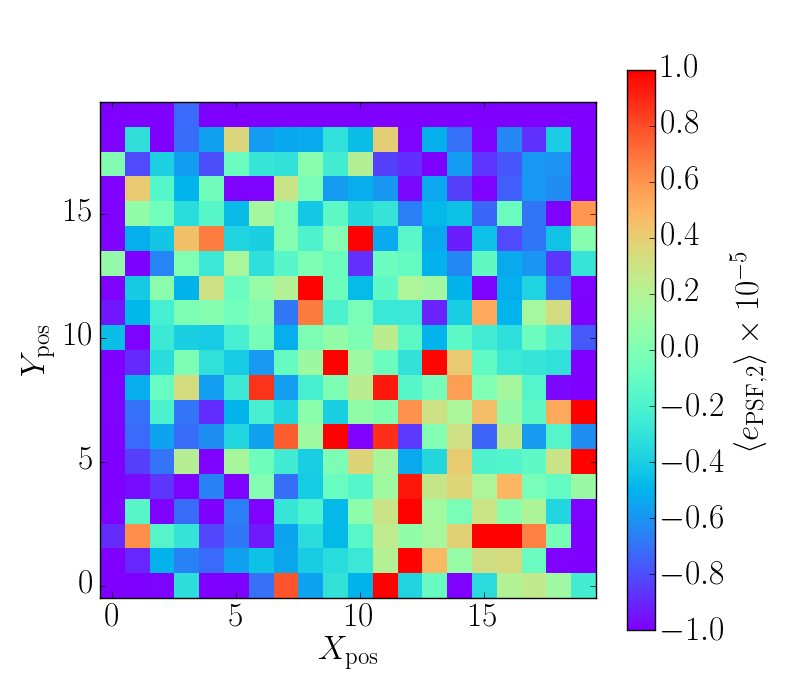
\includegraphics[width=0.49\textwidth]{{Figures/KAll.BlindA.MeanPSFe2_VS_XY.ZBcutNone}.png}
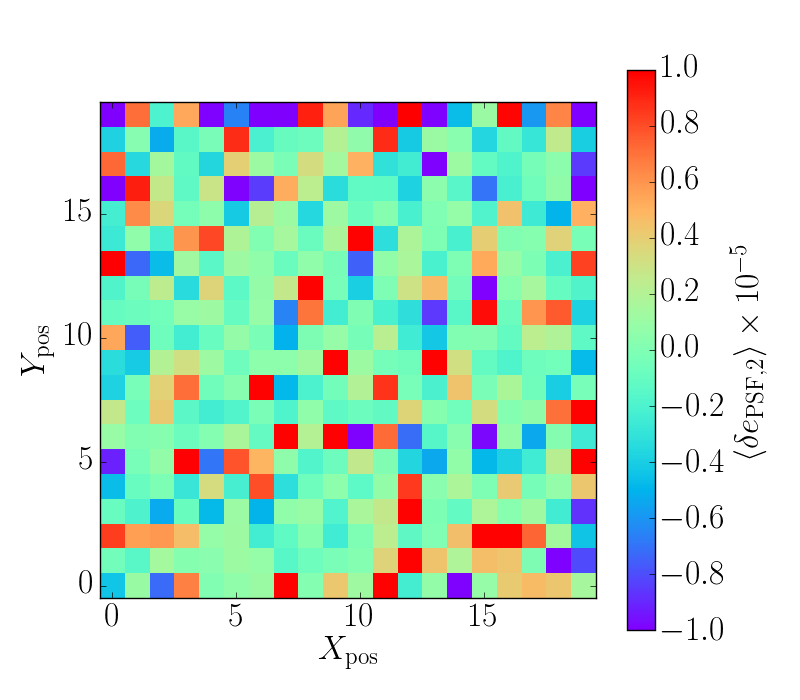
\includegraphics[width=0.49\textwidth]{{Figures/KAll.BlindA.MeandeltaPSFe2_VS_XY.ZBcutNone}.png} \\
\caption{The mean K1000 PSF ellipticity (left panels) and residual, assuming the PSF model with the 4:1 polynomial order (right panels; see equation \ref{eqn:PSFModel_KiDS}), for the $e_1$ and $e_2$ components (upper/lower, respectively), binned by position on the focal plane.} \label{fig:PSFellip_OnTheChip}
\end{center}
\end{figure*} 


    \subsection{PSF tests}
    e.g. shear-PSF size correlation, shear-PSF ellipticity correlation, 
    
    \begin{figure}
\begin{center}
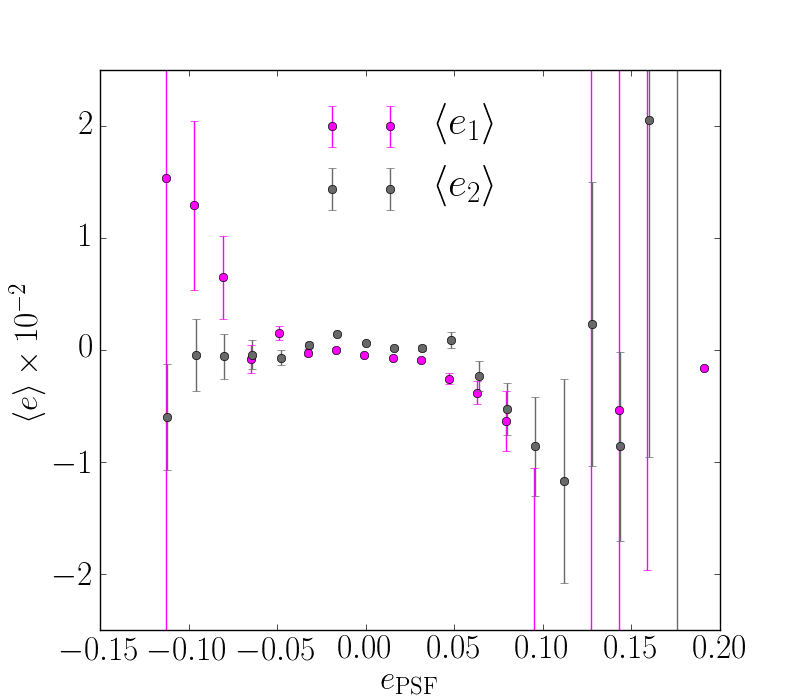
\includegraphics[width=0.49\textwidth]{{Figures/KAll.BlindA.ePSF_VS_e.ZBcutNone}.png} \\
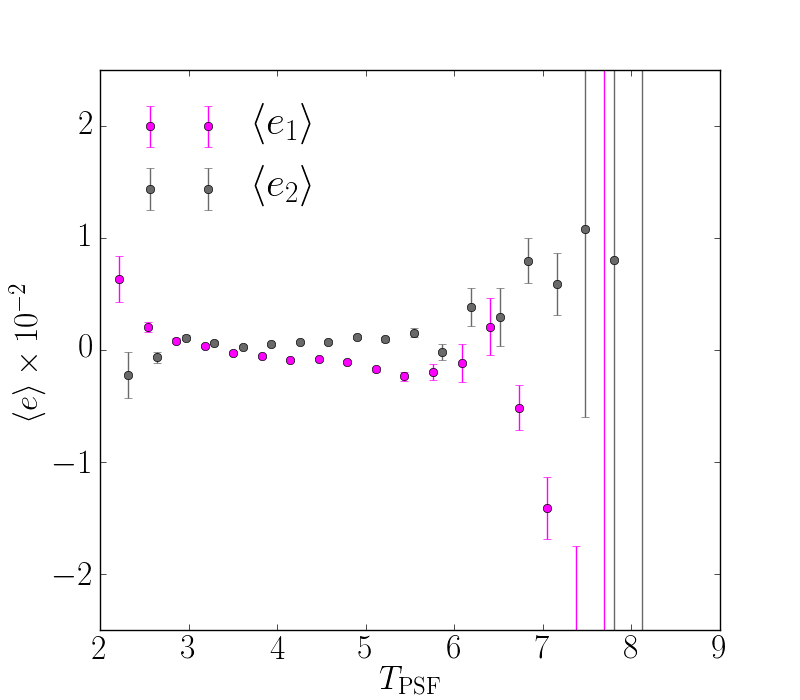
\includegraphics[width=0.49\textwidth]{{Figures/KAll.BlindA.TPSF_VS_e.ZBcutNone}.png}
\caption{The mean galaxy ellipticities binned by the PSF ellipticity (upper) and PSF size (lower), interpolated to the galaxy positions.} \label{fig:Ellip_VS_PSFellip}
\end{center}
\end{figure} 


    \subsection{Galaxy property tests}
    e.g. ellipticity-SNR correlation, ellipticity-galaxy size correlation
    
\begin{figure}
\begin{center}
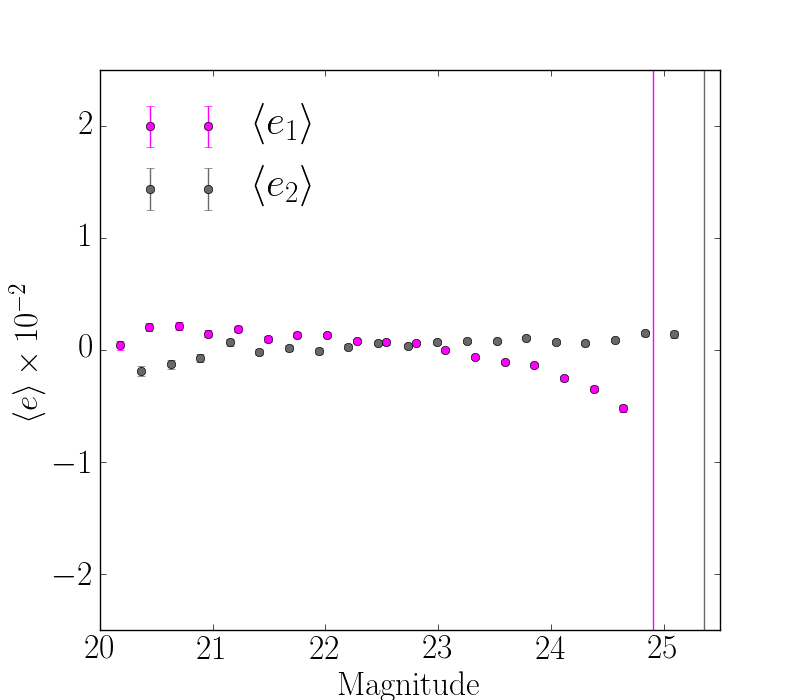
\includegraphics[width=0.49\textwidth]{{Figures/KAll.BlindA.MAG_VS_e.ZBcutNone}.png} \\
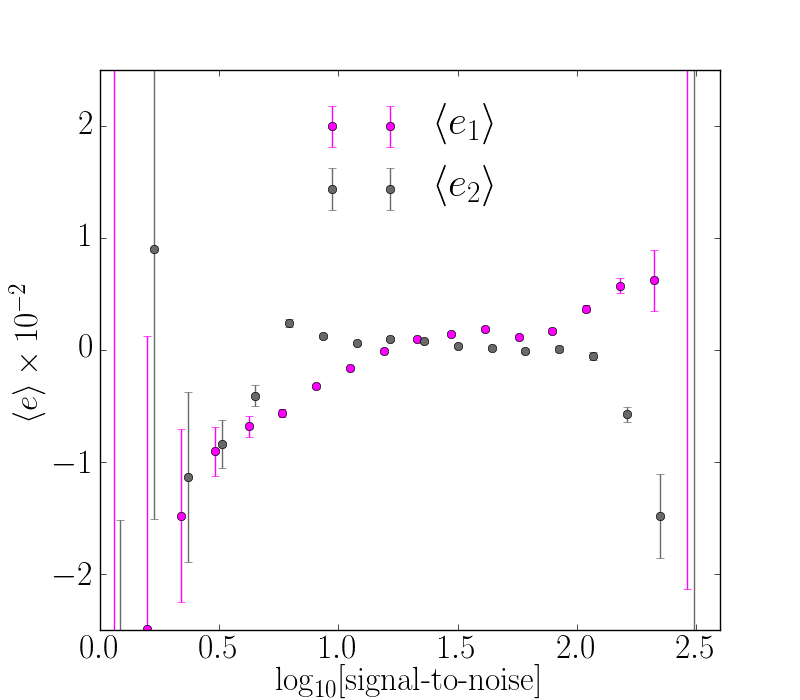
\includegraphics[width=0.49\textwidth]{{Figures/KAll.BlindA.LogSNR_VS_e.ZBcutNone}.png}
\caption{The mean galaxy ellipticities binned by magnitude (upper) and the logarithm of the signal-to-noise (lower).} \label{fig:Ellip_VS_MAG}
\end{center}
\end{figure} 
    
    
    
    \subsection{B-mode tests?}

    \subsection{Internal consistency tests?}
    

\section{Results}

\section{Conclusions and summary}
 
\section{Acknowledgements}
\begin{acknowledgements}
BG, CH acknowledge support from the European Research Council under grant number 647112. 
\end{acknowledgements}

\bibliographystyle{aa} % style aa.bst
\bibliography{references} % your references 


%-------------------------------------------------------------------


\end{document}

